<%= heading2 %>{Plots with pgfplots}

The \href{https://ctan.org/pkg/pgfplots}{pgfplots} package plots functions directly in \LaTeX{}, similar to MATLAB or gnuplot.
Some visual examples are available in the package documentation\footnote{\url{http://texdoc.net/pkg/pgfplots}}.

<%- bexample %>
\begin{figure}[ht]
  \centering
  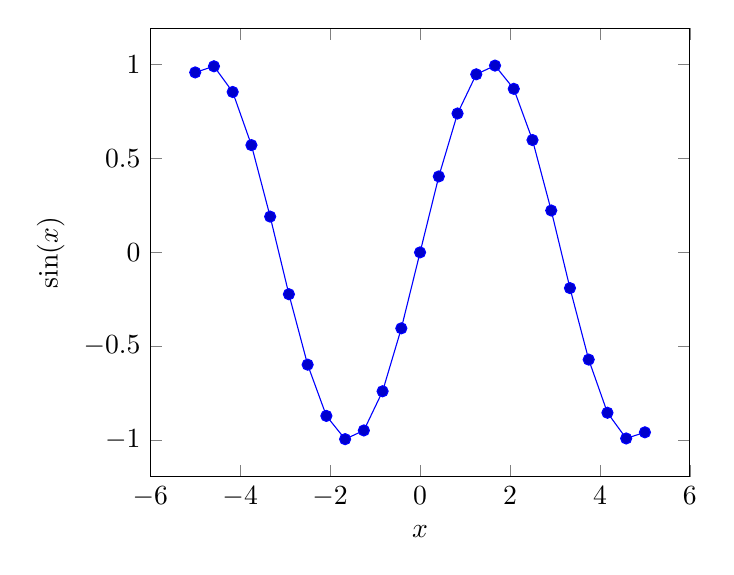
\begin{tikzpicture}
    \begin{axis}[xlabel=$x$, ylabel=$\sin(x)$]
      \addplot {sin(deg(x))};  % Plot the sine function
    \end{axis}
  \end{tikzpicture}
  \caption{Plot of $\sin(x)$ directly inside the figure environment with pgfplots.}
  \label{fig:pgfplots_example}
\end{figure}
<%- eexample %>

Coordinates can also be given explicitly instead of as a function:
<%- bexample %>
\begin{figure}[ht]
  \centering
  \begin{tikzpicture}
    \begin{axis}[xlabel=$x$, ylabel=$y$]
      \addplot coordinates {(0,0) (1,1) (2,4) (3,9)};  % Plot explicit coordinates
    \end{axis}
  \end{tikzpicture}
  \caption{Explicit coordinates plotted with pgfplots.}
  \label{fig:pgfplots_coords}
\end{figure}
<%- eexample %>
